Here we outline the algorithm currently implemented in the code.  The
latest published reference for MAESTRO is the multilevel
paper \cite{multilevel}.  In this description, we make frequent
reference to paper~I \cite{lowMach}, paper~II \cite{lowMach2},
paper~III \cite{lowMach3}, and paper~IV \cite{lowMach4}.




%-----------------------------------------------------------------------------
% Equations Summary
%-----------------------------------------------------------------------------

\section{Summary of the \maestro\ Equation Set}

Here we summarize the equations solved by \maestro.  We refer the reader
to papers~I through IV and the multilevel paper for the derivation
and motivation of the equation set.  (Note: this `traditional' algorithm
uses Strang-splitting for the reactions.  An alternate implementation, using
spectral deferred corrections is outlined in Chapter~\ref{ch:sdc}.)



%-----------------------------------------------------------------------------
% Time Advancement Algorithm
%-----------------------------------------------------------------------------



\section{Time Advancement Algorithm}\label{Sec:Time Advancement Algorithm}
Here is the current description of the algorithm, based from the
description in the multilevel paper.  The initialization has also been
included with more detail than was given in paper III.  The main
driver for a single step of the algorithm is {\tt advance.f90}---refer
to that code to see the sequence of functions called to implement each
step.


\subsection{Notation}

reach\_state

enforce\_hse


\subsection{Single Step}


\begin{description}

%--------------------------------------------------------------------------
% STEP 0
%--------------------------------------------------------------------------

\item[Step 0.] {\em Initialization}

This step remains unchanged from Paper III.  See \S \ref{Sec:Initialization}
for details.  The initialization step only occurs at the beginning of the simulation.  
The initial values for $\Ub^0, \rho^0, (\rho h)^0, X_k^0, T^0, 
\rho_0^0, p_0^0$, and $\overline{\Gamma_1^0}$ are specified from the problem-dependent 
initial conditions.  The initial time step, $\dt^0$, is computed as in 
Paper III.  Finally, initial
values for $w_0^{-\myhalf}, \etarho^{-\myhalf}, \psi^{-\myhalf}, 
\pi^{-\myhalf}, S^0$, and $S^1$ come from a preliminary pass through
the algorithm.  

%--------------------------------------------------------------------------
% STEP 1
%--------------------------------------------------------------------------
\item[Step 1.] {\em React the full state through the first time interval of $\dt / 2.$}

Call {\bf React State}$[\rho^n, (\rho h)^n, X_k^n, T^n, (\rho\Hext)^n, p_0^n]$\\
\phantom{ }\hfill $\rightarrow [\rho^{(1)},(\rho h)^{(1)},X_k^{(1)},T^{(1)},(\rho \omegadot_k)^{(1)},(\rho \Hnuc)^{(1)}]$.

%--------------------------------------------------------------------------
% STEP 2
%--------------------------------------------------------------------------

\item[Step 2.] {\em Compute the provisional time-centered expansion,
  $S^{\nph,\star\star}$, provisional base state velocity,
  $w_0^{\nph,\star}$, and provisional base state velocity forcing.}

\begin{enumerate}
\renewcommand{\theenumi}{{\bf \Alph{enumi}}}

\item Compute $S^{\nph,\star\star}$.  We compute an estimate for the
  time-centered expansion term in the velocity divergence constraint,
  as given in paper~III equation (19),
\begin{equation}
  S =  -\sigma  \sum_k  \xi_k \omegadot_k  + 
  \frac{1}{\rho p_\rho} \sum_k p_{X_k}  {\omegadot}_k  + \sigma \Hnuc + \sigma \Hext 
  + \frac{\sigma}{\rho}\nabla\cdot\kth\nabla T \enskip .
\label{eq:defineS} 
\end{equation}

  For the first time step ($n=0$), we set
\begin{equation}
S^{n+\myhalf,\star\star} = \frac{S^0 + S^1}{2},
\end{equation}
  where $S^1$ is found during initialization.  For other time steps
  $(n \ne 0)$, following \cite{SNe}, we extrapolate
  to the half-time using $S$ at the previous and current
  time levels
\begin{equation}
S^{\nph,\star\star} = S^n + \frac{\dt^n}{2} \frac{S^n - S^{n-1}}{\dt^{n-1}}.
\end{equation}
  Next, compute
\begin{equation}
\overline{S^{\nph,\star\star}} = {\mathrm{\bf Avg}} \left(S^{\nph,\star\star}\right).
\end{equation}

\item Compute $w_0^{\nph,\star}$.
\begin{description}
\item For planar geometry, call\\
{\bf Compute} {\boldmath $w_0$} {\bf Planar}$[\overline{S^{\nph,\star\star}},\overline{\Gamma_1^n},p_0^n,\psi^{n-\myhalf}] \rightarrow [w_0^{\nph,\star}]$.
\item For spherical geometry, call\\
{\bf Compute} {\boldmath $w_0$} {\bf Spherical}$[\overline{S^{\nph,\star\star}},\overline{\Gamma_1^n},\rho_0^n,p_0^n,\etarho^{n-\myhalf}] \rightarrow [w_0^{\nph,\star}]$.
\end{description}

\item Compute the provisional base state velocity forcing, using equation (38)
  from paper~III,
\begin{equation}
-\frac{1}{\rho_0} \frac{\partial \pi_0}{\partial r} = \frac{\partial w_0}{\partial t} + w_0 \frac{\partial w_0}{\partial r}, \label{eq:pizero}
\end{equation}
  with the following discretization:
\begin{equation}
\left ( \frac{1}{\rho_0} \frac{\partial \pi_0}{\partial r} \right )^{n,\star} = -\frac{w_0^{\nph,\star} - w_0^\nmh}{(\dt^n+\dt^{n-1})/2} - w_0^{n,\star} \left(\frac{\partial w_0}{\partial r}\right)^{n,\star},
\end{equation} 
  where $w_0^{n,\star}$ and $(\partial w_0 / \partial r)^{n,\star}$ are defined as
\begin{eqnarray}
w_0^{n,\star} &=& \frac{\dt^{n} w_0^{\nmh} + \dt^{n-1} w_0^{\nph,\star}}{\dt^n+\dt^{n-1}}, \\
\left(\frac{\partial w_0}{\partial r}\right)^{n,\star} &=& \frac{1}{\dt^n+\dt^{n-1}}\left [ \dt^{n} \left(\frac{\partial w_0 }{ \partial r}\right)^{\nmh} + \dt^{n-1} \left(\frac{\partial w_0 }{ \partial r}\right)^{\nph,\star} \right ].\nonumber \\
\end{eqnarray}
  If $n=0$, we use $\dt^{-1} = \dt^0$.
\end{enumerate}

%--------------------------------------------------------------------------
% STEP 3
%--------------------------------------------------------------------------
\item[Step 3.] {\em Construct the provisional time-centered advective velocity on 
edges, $\uadvone$.}

The local velocity field is described by paper III equation (37),
\begin{equation}
\frac{\partial\Ubt}{\partial t} = 
- \left(\Ubt+w_0\right) \cdot \nabla \Ubt
- \left(\Ubt \cdot \eb_r\right) \frac{\partial w_0}{\partial r} \eb_r
- \frac{1}{\rho} \nabla\pi
+ \frac{1}{\rho_0} \frac{\partial \pizero}{\partial r} \eb_r
- \frac{(\rho-\rhozero)}{\rho} \; g \; \eb_r  \label{eq:utildeupd}  \enskip .
\end{equation}
From this, we compute time-centered edge 
velocities, $\uadvonedag$, using 
$\Ub = \Ubt^n + w_0^{\nph,\star}$.  The $\dagger$ superscript refers to the 
fact that the predicted velocity field does not satisfy the divergence 
constraint.  We then construct $\uadvone$ from $\uadvonedag$
using a MAC projection, as described in detail in Appendix B of Paper III.  
We note that $\uadvone$ satisfies the discrete version of
$\overline{(\uadvone\cdot\eb_r)}=0$ as well as
\begin{eqnarray}
\nabla \cdot \left(\beta_0^n \uadvone\right) &=& \beta_0^n \left(S^{\nph,\star\star} - \overline{S^{\nph,\star\star}}\right),\\
 \beta_0^n &=& \beta_0 \left(\rho_0^n, p_0^n, \overline{\Gamma_1^n}\right),
\end{eqnarray}
where $\beta_0$ is computed as described in Appendix C of Paper III.

%--------------------------------------------------------------------------
% STEP 4
%--------------------------------------------------------------------------
\item[Step 4.] {\em Advect the base state and full state through a time interval of $\dt.$}

\begin{enumerate}
\renewcommand{\theenumi}{{\bf \Alph{enumi}}}

\item Update $\rho_0$, saving the time-centered density at radial edges by calling

{\bf Advect Base Density}$[\rho_0^{n},w_0^{\nph,\star}] \rightarrow [\rho_0^{(2a),\star}, \rho_0^{\nph,\star,\pred}]$.

\item Update $(\rho X_k)$ using a discretized version of the species 
continuity equation,
\begin{equation}
\frac{\partial (\rho X_k)}{\partial t} + \nabla \cdot (\Ub \rho X_k) = 0 \enskip .
\label{eq:species}
\end{equation}
where we omit the reaction terms, which were already 
accounted for in {\bf React State}.  The update consists of two steps:

\begin{enumerate}
\renewcommand{\labelenumii}{{\bf \roman{enumii}}.}

\item Compute the time-centered species edge states, $(\rho X_k)^{\nph,\star,\pred}$,
  for the conservative update of $(\rho X_k)^{(1)}$.  

  There are a variety of choices of quantities to predict to the
  edges (controlled by {\tt species\_pred\_type}---see Chapter~\ref{ch:pert}).
  By default, we use the equations 
\begin{eqnarray}
\frac{\partial\rho'}{\partial t} &=& -\Ub\cdot\nabla\rho' - 
     \rho'\nabla\cdot\Ub - \nabla\cdot\left(\rho_0\Ubt\right),
     \label{eq:Perturbational Density}  \\
\frac{\partial X_k}{\partial t} &=& -\Ub\cdot\nabla X_k + 
     \omegadot_k. \label{eq:Primitive Species}
\end{eqnarray}
  to
  predict $\rho^{'(1)} = \rho^{(1)} - \rho_0^n$ and 
  $X_k^{(1)} = (\rho  X_k)^{(1)} / \rho^{(1)}$ to time-centered edges using 
  $\Ub = \uadvone+w_0^{\nph,\star}\eb_r$, yielding $\rho^{'\nph,\star,\pred}$ 
  and $X_k^{\nph,\star,\pred}$.
  We convert the perturbational density to full state density using
\begin{equation}
\rho^{\nph,\star,\pred} = \rho^{'\nph,\star,\pred} + \frac{\rho_0^n + \rho_0^{(2a),\star}}{2},
\end{equation}
  where the base state density terms are mapped to Cartesian edges.
  Then,\\
  $(\rho X_k)^{\nph,\star,\pred} = (\rho^{\nph,\star,\pred}X_k^{\nph,\star,\pred})$.

\item Evolve $(\rho X_k)^{(1)} \rightarrow (\rho X_k)^{(2),\star}$ using
\begin{eqnarray}
(\rho X_k)^{(2),\star} &=& (\rho X_k)^{(1)} \nonumber \\
&& - \dt \left\{ \nabla \cdot \left[ \left(\uadvone+w_0^{\nph,\star} \eb_r\right) (\rho X_k)^{\nph,\star,\pred} \right] \right\},\nonumber \\
\end{eqnarray}
\begin{equation}
\rho^{(2),\star} = \sum_k (\rho X_k)^{(2),\star},
\qquad
X_k^{(2),\star} = (\rho X_k)^{(2),\star} / \rho^{(2),\star}.
\end{equation}

\end{enumerate}

\item Define a radial edge-centered $\etarho^{\nph,\star}$.

\begin{description}
\item For planar geometry, since $\etarho = \overline{\rho'(\Ub\cdot\eb_r)} = \overline{\rho(\Ub\cdot\eb_r)}-\overline{\rho_0(\Ub\cdot\eb_r}) = \overline{\rho(\Ub\cdot\eb_r)} - \rho_0w_0$,
\begin{eqnarray}
 \etarho^{\nph,\star} &=&  {\rm {\bf Avg}} \sum_k \left[ \left(\uadvone \cdot \eb_r + w_0^{\nph,\star}\right) (\rho X_k)^{\nph,\star,\pred} \right]\nonumber\\
&& - w_0^{\nph,\star} \rho_0^{\nph,\star,\pred},
\end{eqnarray}
\item For spherical geometry, first construct 
$\etarho^{{\rm cart},\nph,\star} = [\rho'(\Ub\cdot\eb_r)]^{\nph,\star}$ on Cartesian cell centers using:
\begin{eqnarray}
\etarho^{{\rm cart},\nph,\star} &=& \left[\left(\frac{\rho^{(1)}+\rho^{(2),\star}}{2}\right)-\left(\frac{\rho_0^n+\rho_0^{(2a),\star}}{2}\right)\right] \nonumber \\
&&\cdot \left( \uadvone \cdot \eb_r  + w_0^{\nph,\star}\right).
\end{eqnarray}
Then,
\begin{equation}
\etarho^{\nph,\star} = {\rm {\bf Avg}}\left(\etarho^{{\rm cart},\nph,\star}\right).
\end{equation}
This gives a radial cell-centered $\etarho^{\nph,\star}$.  To get
$\etarho^{\nph,\star}$ at radial edges, average the two neighboring
radial cell-centered values.
\end{description}

\item Correct $\rho_0$ by setting $\rho_0^{n+1,\star} =$ {\bf Avg}$(\rho^{(2),\star})$.

\item Update $p_0$ by calling 
{\bf Enforce HSE}$[p_0^n,\rho_0^{n+1,\star}] \rightarrow [p_0^{n+1,\star}]$.

\item Compute $\psi^{\nph,\star}$.
\begin{description}
\item For planar geometry,
\begin{equation}
\psi_j^{\nph,\star} = \frac{1}{2} \left(\eta_{\rho,j-\myhalf}^{\nph,\star} 
+ \eta_{\rho,j+\myhalf}^{\nph,\star}\right) g.
\end{equation}
\item For spherical geometry, first compute:
\begin{eqnarray}
\overline{\Gamma_1^{(1)}} &=& {\rm{\bf Avg}} \left[ \Gamma_1\left(\rho^{(1)}, p_0^{n}, X_k^{(1)}\right) \right]  , \\
\overline{\Gamma_1^{(2),\star}} &=& {\rm{\bf Avg}} \left[ \Gamma_1\left(\rho^{(2),\star}, p_0^{n+1,\star}, X_k^{(2),\star}\right) \right].
\end{eqnarray}
Then, define $\psi^{\nph,\star}$ using equation (\ref{eq:psi def})
\begin{eqnarray}
\psi_j^{\nph,\star} 
&=& \left(\frac{\overline{\Gamma_1^{(1)}}+\overline{\Gamma_1^{(2),\star}}}{2}\right)_j
\left(\frac{p_0^n+p_0^{n+1,\star}}{2}\right)_j \nonumber \\
&& \left \{ \overline{S_j^{\nph,\star}} - \frac{1}{r_j^2} \left [ \left(r^2 w_0^{\nph,\star}\right)_{j+\myhalf} - \left(r^2 w_0^{\nph,\star}\right)_{j-\myhalf} \right ] \right \}.\nonumber \\
\end{eqnarray}
\end{description}

\item Update $(\rho h)_0$.  First, compute $(\rho h)_0^n = $ {\bf Avg}$[(\rho h)^{(1)}]$.
Then, call\\
{\bf Advect Base Enthalpy}$[(\rho h)_0^{n}, w_0^{\nph,\star}, \psi^{\nph,\star}] \rightarrow [(\rho h)_0^{n+1,\star}]$.

\item Update the enthalpy using a discretized version of the enthalpy
evolution equation, again omitting the reaction and heating terms
since we already accounted for
them in {\bf React State}.  This equation takes the form:
\begin{equation}
\frac{\partial (\rho h)}{\partial t}  = - \nabla \cdot (\Ub \rho h) + \psi + (\Ubt \cdot \eb_r) \frac{\partial p_0}{\partial r}.
\end{equation}
For spherical geometry, we solve the
analytically equivalent form,
\begin{equation}
\frac{\partial (\rho h)}{\partial t}  = - \nabla \cdot (\Ub \rho h) + \psi + \nabla \cdot (\Ubt p_0) - p_0 \nabla \cdot \Ubt,
\end{equation}
which experience has shown to minimize the drift from thermodynamic
equilibrium.  The update consists of two steps:

\begin{enumerate}
\renewcommand{\labelenumii}{{\bf \roman{enumii}}.}

\item Compute the time-centered enthalpy edge state, $(\rho h)^{\nph,\star,\pred},$
  for the conservative update of $(\rho h)^{(1)}$.  There are a variety
   of quantities that we can predict to the interfaces here (controlled
   by {\tt enthalpy\_pred\_type}---see Chapter~\ref{ch:pert}).  For
   the default case, we use the perturbational
  enthalpy equation, neglecting reactions,
\begin{equation}
\frac{\partial(\rho h)'}{\partial t} = -\Ub\cdot\nabla(\rho h)' - 
   (\rho h)'\nabla\cdot\Ub - \nabla\cdot\left[(\rho h)_0\Ubt\right] + \Ubt\cdot\nabla p_0 
    \label{eq:Perturbational Enthalpy}.
\end{equation}
  to predict
  $(\rho h)' = (\rho h)^{(1)} - (\rho h)_0^n$ to time-centered edges, 
  using $\Ub = \uadvone+w_0^{\nph,\star} \eb_r$,
  yielding $(\rho h)^{'\nph,\star,\pred}$.  We convert the perturbational 
  enthalpy to a full state enthalpy using
\begin{equation}
(\rho h)^{\nph,\star,\pred} = (\rho h)^{'\nph,\star,\pred} + \frac{(\rho h)_0^n + (\rho h)_0^{n+1,\star}}{2}.
\end{equation}
  For planar geometry, we map $(\rho h)_0$ directly to Cartesian edges.
  In spherical geometry, our experience has shown that a slightly different
  approach leads to reduced discretization errors.  We first map 
  $h_0 \equiv (\rho h)_0/\rho_0$ and $\rho_0$ to Cartesian edges separately, 
  and then multiply these terms to get $(\rho h)_0$.

\item Evolve $(\rho h)^{(1)} \rightarrow (\rho h)^{(2),\star}$.
\begin{description}
\item For planar geometry,
\begin{eqnarray}
(\rho h)^{(2),\star} 
&=& (\rho h)^{(1)} \nonumber \\
&&- \dt \left\{ \nabla \cdot \left[ \left(\uadvone+w_0^{\nph,\star} \eb_r\right) (\rho h)^{\nph,\star,\pred} \right] \right\} \nonumber \\ 
&& + \dt \left(\uadvone \cdot \eb_r\right) \left(\frac{\partial p_0}{\partial r} \right)^{n} + \dt \psi^{\nph,\star},
\end{eqnarray}

\item For spherical geometry,
\begin{eqnarray}
(\rho h)^{(2),\star} 
&=& (\rho h)^{(1)} \nonumber \\
&&- \dt \left\{ \nabla \cdot \left[ \left(\uadvone+w_0^{\nph,\star} \eb_r\right) (\rho h)^{\nph,\star,\pred} \right] \right\} \nonumber \\ 
&& + \dt \left \{ \nabla \cdot \left (\uadvone p_0^{n} \right ) - p_0^{n} \nabla \cdot \uadvone \right \} \nonumber \\
&&+ \dt \psi^{\nph,\star},
\end{eqnarray}
\end{description}

\end{enumerate}

Then, for each Cartesian cell where $\rho^{(2),\star} < \rho_\mathrm{cutoff}$,
we recompute enthalpy using
\begin{equation}
(\rho h)^{(2),\star} = \rho^{(2),\star}h\left(\rho^{(2),\star},p_0^{n+1,\star},X_k^{(2),\star}\right).
\end{equation}

\item Update the temperature using the equation of state:
$T^{(2),\star} = 
  T(\rho^{(2),\star}, h^{(2),\star}, X_k^{(2),\star})$ (planar geometry) or
$T^{(2),\star} = 
  T(\rho^{(2),\star}, p_0^{n+1,\star}, X_k^{(2),\star})$ (spherical geometry).
\end{enumerate}

%--------------------------------------------------------------------------
% STEP 5
%--------------------------------------------------------------------------
\item[Step 5.] {\em React the full state through a second time interval of $\dt / 2.$}

Call {\bf React State}$[ \rho^{(2),\star},(\rho h)^{(2),\star}, X_k^{(2),\star}, T^{(2),\star}, 
(\rho\Hext)^{(2),\star}, p_0^{n+1,\star}]$\\
\phantom{ }\hfill$\rightarrow [ \rho^{n+1,\star},(\rho h)^{n+1,\star}, X_k^{n+1,\star}, T^{n+1,\star}, (\rho \omegadot_k)^{(2),\star}, (\rho \Hnuc)^{(2),\star} ].$

%--------------------------------------------------------------------------
% STEP 6
%--------------------------------------------------------------------------
\item[Step 6.] {\em Compute the time-centered expansion, $S^{\nph,\star}$, base state
velocity, $w_0^{\nph}$, and base state velocity forcing.}

\begin{enumerate}
\renewcommand{\theenumi}{{\bf \Alph{enumi}}}

\item Compute $S^{\nph,\star}$.  First, compute $S^{n+1,\star}$ with
\begin{equation}
S^{n+1,\star} =  -\sigma  \sum_k  \xi_k  (\omegadot_k)^{(2),\star}  + \frac{1}{\rho^{n+1,\star} p_\rho} \sum_k p_{X_k}  ({\omegadot}_k)^{(2),\star} + \sigma \Hnuc^{(2),\star} + \sigma \Hext^{(2),\star},
\end{equation}
  where $(\omegadot_k)^{(2),\star} = (\rho \omegadot_k)^{(2),\star} /
  \rho^{(2),\star}$ and the thermodynamic quantities are defined using
  $\rho^{n+1,\star}, X_k^{n+1,\star},$ and $T^{n+1,\star}$ as inputs to
  the equation of state.  Then, define
\begin{equation}
\overline{S^{\nph,\star}} = {\mathrm{\bf Avg}} (S^{\nph,\star}),
\qquad
 S^{\nph.\star} = \frac{S^n + S^{n+1,\star}}{2},
\end{equation}
\item Compute $w_0^{\nph}$.  First, define
\begin{equation}
\overline{\Gamma_1^{\nph,\star}} = \frac{\overline{\Gamma_1^n} + \overline{\Gamma_1^{n+1,\star}}}{2}, 
\quad
\rho_0^{\nph,\star} = \frac{\rho_0^{n} + \rho_0^{n+1,\star}}{2},
\quad
p_0^{\nph,\star} = \frac{p_0^{n} + p_0^{n+1,\star}}{2},
\end{equation}
  with
\begin{equation}
 \overline{\Gamma_1^{n+1,\star}} = {\rm{\bf Avg}} \left[ \Gamma_1\left(\rho^{n+1,\star}, p_0^{n+1,\star}, X_k^{n+1,\star}\right) \right].
\end{equation}
\begin{description}
\item For planar geometry, call\\
{\bf Compute} {\boldmath $w_0$} {\bf Planar}$[\overline{S^{\nph,\star}},\overline{\Gamma_1^{\nph,\star}},p_0^{\nph,\star},\psi^{\nph,\star}]\rightarrow [w_0^{\nph}]$.
\item For spherical geometry, call\\
{\bf Compute} {\boldmath $w_0$} {\bf Spherical}$[\overline{S^{\nph,\star}},\overline{\Gamma_1^{\nph,\star}},\rho_0^{\nph,\star},p_0^{\nph,\star},\etarho^{\nph,\star}]$\\
\phantom{ }\hfill$\rightarrow [w_0^{\nph}]$.
\end{description}

\item Compute the base state velocity forcing.  Rearrange equation (\ref{eq:pizero}),
\begin{equation}
\left ( \frac{1}{\rho_0} \frac{\partial \pi_0}{\partial r} \right )^n = 
-\frac{w_0^{\nph} - w_0^\nmh}{\myhalf(\dt^n+\dt^{n-1})} 
- w_0^n \left(\frac{\partial w_0}{\partial r}\right)^n,
\end{equation}
  where $w_0^{n}$ and $(\partial w_0 / \partial r)^{n}$ are defined as
\begin{eqnarray}
w_0^n &=& \frac{\dt^{n} w_0^{\nmh} + \dt^{n-1} w_0^{\nph}}{\dt^n+\dt^{n-1}}, \\
\left(\frac{\partial w_0}{\partial r}\right)^{n} &=& \frac{1}{\dt^n+\dt^{n-1} } \left [ \dt^{n} \left(\frac{\partial w_0 }{ \partial r}\right)^{\nmh} + \dt^{n-1} \left(\frac{\partial w_0 }{ \partial r}\right)^{\nph} \right ].\nonumber \\
\end{eqnarray}
  If $n=0$, we use $\dt^{-1} = \dt^0$.

\end{enumerate}

%--------------------------------------------------------------------------
% STEP 7
%--------------------------------------------------------------------------
\item[Step 7.] {\em Construct the time-centered advective velocity on edges, $\uadvtwo$.}

The procedure to construct $\uadvtwodag$ is identical to the procedure
for computing $\uadvonedag$ in {\bf Step 3}, but uses 
the updated values $w_0^{\nph}$ and $\pi_0^n$ rather than $w_0^{\nph,\star}$ 
and $\pi_0^{n,\star}$.  We note that $\uadvtwo$ satisfies the discrete version of
$\overline{(\uadvtwo\cdot\eb_r)}=0$ as well as
\begin{equation}
\nabla \cdot \left(\beta_0^{\nph,\star} \uadvtwo\right) =
\beta_0^{\nph,\star}\left(S^{\nph,\star} - \overline{S^{\nph,\star}}\right),
\end{equation}
\begin{equation}
\beta_0^{\nph,\star} = \frac{ \beta_0^n +  \beta_0^{n+1,\star} }{2};
\qquad
 \beta_0^{n+1,\star} = \beta_0 \left(\rho_0^{n+1,\star}, p_0^{n+1,\star}, \overline{\Gamma_1^{n+1,\star}}\right).
\end{equation}

%--------------------------------------------------------------------------
% STEP 8
%--------------------------------------------------------------------------
\item[Step 8.] {\em Advect the base state and full state through a time interval of $\dt.$}

\begin{enumerate}
\renewcommand{\theenumi}{{\bf \Alph{enumi}}}

\item Update $\rho_0$, saving the time-centered density at radial edges by calling

{\bf Advect Base Density}$[\rho_0^{n},w_0^{\nph}] \rightarrow [\rho_0^{(2a)}, \rho_0^{\nph,\pred}]$.

\item Update $(\rho X_k)$.  This step is identical to {\bf Step 4B} except we use
  the updated values $w_0^{\nph}, \uadvtwo$, and $\rho_0^{(2a)}$ rather than 
  $w_0^{\nph,\star}, \uadvone$, and $\rho_0^{(2a),\star}$.  In particular:

\begin{enumerate}
\renewcommand{\labelenumii}{{\bf \roman{enumii}}.}

\item Compute the time-centered species edge states, $(\rho X_k)^{\nph,\pred}$,
  for the conservative update of $(\rho X_k)^{(1)}$.  We use equations 
  (\ref{eq:Perturbational Density}) and (\ref{eq:Primitive Species}) to 
  predict $\rho^{'(1)} = \rho^{(1)} - \rho_0^n$ and 
  $X_k^{(1)} = (\rho  X_k)^{(1)} / \rho^{(1)}$ to time-centered edges
  with $\Ub = \uadvtwo+w_0^{\nph} \eb_r$,
  yielding $\rho^{'\nph,\pred}$ and $X_k^{\nph,\pred}$.  
  We convert the perturbational density to a full state density using
\begin{equation}
\rho^{\nph,\pred} = \rho^{'\nph,\pred} + \frac{\rho_0^n + \rho_0^{(2a)}}{2}.
\end{equation}
  Then, $(\rho X_k)^{\nph,\pred} = (\rho^{\nph,\pred}X_k^{\nph,\pred})$.

\item Evolve $(\rho X_k)^{(1)} \rightarrow (\rho X_k)^{(2)}$ using
\begin{equation}
(\rho X_k)^{(2)} = (\rho X_k)^{(1)} 
- \dt \left\{ \nabla \cdot \left[\left(\uadvtwo+w_0^{\nph} \eb_r\right)  
(\rho X_k)^{\nph,\pred} \right] \right\},
\end{equation}
\begin{equation}
\rho^{(2)} = \sum_k (\rho X_k)^{(2)},
\qquad
X_k^{(2)} = (\rho X_k)^{(2)} / \rho^{(2)}.
\end{equation}

\end{enumerate}

\item Define a radial edge-centered $\etarho^{\nph}$.
\begin{description}
\item For planar geometry,
\begin{eqnarray}
 \etarho^{\nph} &=& {\rm {\bf Avg}} \sum_k \left [\left(\uadvtwo \cdot \eb_r + w_0^{\nph}\right) (\rho X_k)^{\nph,\pred} \right] \nonumber \\
&&- w_0^{\nph} \rho_0^{\nph,\pred},
\end{eqnarray}
\item For spherical geometry, first construct 
$\etarho^{{\rm cart},\nph} = [\rho'(\Ub\cdot\eb_r)]^{\nph}$ on Cartesian
  cell centers using:
\begin{equation}
\etarho^{{\rm cart},\nph} = \left[\left(\frac{\rho^{(1)}+\rho^{(2)}}{2}\right)-\left(\frac{\rho_0^n+\rho_0^{(2a)}}{2}\right)\right] \left(\uadvtwo \cdot \eb_r + w_0^{\nph}\right).
\end{equation}
Then,
\begin{equation}
\etarho^{\nph} = {\rm {\bf Avg}}\left(\etarho^{{\rm cart},\nph}\right).
\end{equation}
This gives a radial cell-centered $\etarho^{\nph}$.  To get
$\etarho^{\nph}$ at radial edges, average the two neighboring
cell-centered values.
\end{description}

\item Correct $\rho_0$ by setting $\rho_0^{n+1} =$ {\bf Avg}$(\rho^{(2)})$.

\item Update $p_0$ by calling
{\bf Enforce HSE}$[p_0^n,\rho_0^{n+1}] \rightarrow [p_0^{n+1}]$.

\item Compute $\psi^{\nph}$.
\begin{description}
\item For planar geometry, 
\begin{equation}
\psi_j^{\nph} = \frac{1}{2} \left(\eta_{\rho,j-\myhalf}^{\nph} 
+ \eta_{\rho,j+\myhalf}^{\nph}\right) g.
\end{equation}
\item For spherical geometry, first compute:
\begin{equation}
\overline{\Gamma_1^{(2)}} = {\rm{\bf Avg}} \left[ \Gamma_1\left(\rho^{(2)}, p_0^{n+1}, 
X_k^{(2)}\right) \right].
\end{equation}
Then, define $\psi^{\nph}$ using equation (\ref{eq:psi def}):
\begin{eqnarray}
\psi_j^{\nph} 
&=& \left(\frac{\overline{\Gamma_1^{(1)}}+\overline{\Gamma_1^{(2)}}}{2}\right)_j \left(\frac{p_0^n+p_0^{n+1}}{2}\right)_j \nonumber \\
&& \left \{ \overline{S_j^{\nph}} - \frac{1}{r_j^2} \left [ \left(r^2 w_0^{\nph}\right)_{j+\myhalf} - \left(r^2 w_0^{\nph}\right)_{j-\myhalf} \right ] \right \}.
\end{eqnarray}
\end{description}

\item Update $(\rho h)_0$ by calling 
{\bf Advect Base Enthalpy}$[(\rho h)_0^n, w_0^{\nph}, \psi^{\nph}] \rightarrow [(\rho h)_0^{n+1}]$.

\item Update the enthalpy.  This step is identical to {\bf Step 4H} except we use
  the updated values $w_0^{\nph}, \uadvtwo, \rho_0^{n+1}, (\rho h)_0^{n+1}, p_0^{n+\myhalf}$, 
  and $\psi^{n+\myhalf}$ rather than\\
  $w_0^{\nph,\star}, \uadvone, \rho_0^{n+1,\star}, (\rho h)_0^{n+1,\star}, p_0^n$, 
  and $\psi^{n+\myhalf,\star}$.  In particular:

\begin{enumerate}
\renewcommand{\labelenumii}{{\bf \roman{enumii}}.}

\item Compute the time-centered enthalpy edge state, $(\rho h)^{\nph,\pred},$
  for the conservative update of $(\rho h)^{(1)}$.  We use equation 
  (\ref{eq:Perturbational Enthalpy}) to predict
  $(\rho h)' = (\rho h)^{(1)} - (\rho h)_0^n$ to time-centered edges
  with $\Ub = \uadvtwo+w_0^{\nph} \eb_r$,
  yielding $(\rho h)^{'\nph,\pred}$.  
  We convert the perturbational enthalpy to a full state enthalpy using
\begin{equation}
(\rho h)^{\nph,\pred} = (\rho h)^{'\nph,\pred} + \frac{(\rho h)_0^n + (\rho h)_0^{n+1}}{2}.
\end{equation}

\item Evolve $(\rho h)^{(1)} \rightarrow (\rho h)^{(2)}$.
\begin{description}
\item For planar geometry,
\begin{eqnarray}
(\rho h)^{(2)} 
&=& (\rho h)^{(1)} - \dt \left\{ \nabla \cdot \left[ \left(\uadvtwo+w_0^{\nph} \eb_r\right)  (\rho h)^{\nph,\pred} \right] \right\} \nonumber \\
&& + \dt \left(\uadvtwo \cdot \eb_r\right) \left(\frac{\partial p_0}{\partial r} \right)^\nph + \dt \psi^{\nph},
\end{eqnarray}

\item For spherical geometry,
\begin{eqnarray}
(\rho h)^{(2)} 
&=& (\rho h)^{(1)} - \dt \left\{ \nabla \cdot \left[ \left(\uadvtwo+w_0^{\nph} \eb_r\right)  (\rho h)^{\nph,\pred} \right] \right\} \nonumber \\
&& + \dt \left[ \nabla \cdot \left (\uadvtwo p_0^{\nph} \right ) - p_0^{\nph} \nabla \cdot \uadvtwo \right] + \dt \psi^{\nph},\nonumber \\
\end{eqnarray}
\end{description}
where $p_0^\nph$ is defined as $p_0^\nph = (p_0^n+p_0^{n+1})/2$.

\end{enumerate}

Then, for each Cartesian cell where $\rho^{(2)} < \rho_\mathrm{cutoff}$, we recompute enthalpy using
\begin{equation}
(\rho h)^{(2)} = \rho^{(2)}h\left(\rho^{(2)},p_0^{n+1},X_k^{(2)}\right).
\end{equation}

\item Update the temperature using the equation of state:
$T^{(2)} = 
   T(\rho^{(2)}, h^{(2)}, X_k^{(2)})$ (planar geometry) or
$T^{(2)} = 
   T(\rho^{(2)}, p_0^{n+1}, X_k^{(2)})$ (spherical geometry).
\end{enumerate}

%--------------------------------------------------------------------------
% STEP 9
%--------------------------------------------------------------------------
\item[Step 9.] {\em React the full state through a second time interval of $\dt / 2.$}

Call {\bf React State}$[\rho^{(2)},(\rho h)^{(2)}, X_k^{(2)},T^{(2)}, (\rho\Hext)^{(2)}, p_0^{n+1}]$\\
\phantom{ }\hfill$\rightarrow [\rho^{n+1}, (\rho h)^{n+1}, X_k^{n+1}, T^{n+1}, (\rho \omegadot_k)^{(2)}, (\rho \Hnuc)^{(2)} ].$  

%--------------------------------------------------------------------------
% STEP 10
%--------------------------------------------------------------------------
\item[Step 10.] {\em Define the new time expansion, $S^{n+1}$, and $\overline{\Gamma_1^{n+1}}$.}

\begin{enumerate}
\renewcommand{\theenumi}{{\bf \Alph{enumi}}}
\item Define
\begin{equation}
  S^{n+1} =  -\sigma  \sum_k  \xi_k (\omegadot_k)^{(2)}  + \sigma \Hnuc^{(2)} +
  \frac{1}{\rho^{n+1} p_\rho} \sum_k p_{X_k}  ({\omegadot}_k)^{(2)}  
   + \sigma \Hext^{(2)},
\end{equation}
where $(\omegadot_k)^{(2)} = (\rho \omegadot_k)^{(2)} / \rho^{(2)}$
and the thermodynamic quantities are defined using $\rho^{n+1}$,
$X_k^{n+1}$, and $T^{n+1}$ as inputs to the equation of state.
Then, compute
\begin{equation}
\overline{S^{n+1}} = {\mathrm{\bf Avg}} (S^{n+1}).
\end{equation}

\item Define
\begin{equation}
\overline{\Gamma_1^{n+1}} = {\rm{\bf Avg}}\left[\Gamma_1\left(\rho^{n+1}, p_0^{n+1}, 
X_k^{n+1}\right) \right].
\end{equation}

\end{enumerate}


%--------------------------------------------------------------------------
% STEP 11
%--------------------------------------------------------------------------
\item[Step 11.] {\em Update the velocity}.  

First, we compute the time-centered edge velocities, $\Ubt^{\nph,\pred}$.
Then, we define
\begin{equation}
\rho^\nph = \frac{\rho^n + \rho^{n+1}}{2}, \qquad \rho_0^\nph = \frac{\rho_0^n + \rho_0^{n+1}}{2}.
\end{equation}
We update the velocity field $\Ubt^n$ to $\Ubt^{n+1,\dagger}$ by discretizing 
equation (\ref{eq:utildeupd}) as
\begin{eqnarray}
\Ubt^{n+1,\dagger} 
&=& \Ubt^n - \dt \left[\left(\uadvtwo+ w_0^{\nph} \eb_r\right) \cdot \nabla \Ubt^{\nph,\pred} \right] \nonumber \\
&&- \dt \left(\uadvtwo \cdot \eb_r\right)  \left(\frac{\partial w_0}{\partial r} \right)^\nph \eb_r \nonumber \\
&& + \dt \left[ - \frac{1}{\rho^\nph} \mathbf{G} \pi^\nmh + \left(\frac{1}{\rho_0}\frac{\partial\pi_0}{\partial r}\right)^n \eb_r - \frac{\left(\rho^\nph-\rho_0^\nph\right)}{\rho^\nph} g^{\nph} \eb_r \right],\nonumber \\
\end{eqnarray}
where $\mathbf{G}$ approximates a cell-centered gradient from nodal
data.  Again, the $\dagger$ superscript refers 
to the fact that the updated velocity does not satisfy the divergence 
constraint.

Finally, we use an approximate nodal projection to define $\Ubt^{n+1}$
from $\Ubt^{n+1,\dagger},$  such that $\Ubt^{n+1}$ approximately
satisfies 
\begin{equation}
\nabla \cdot \left(\beta_0^{\nph} \Ubt^{n+1} \right) 
= \beta_0^{\nph} \left(S^{n+1} - \overline{S^{n+1}} \right),
\end{equation}
where $\beta_0^{\nph}$ is defined as
\begin{equation}
\beta_0^{\nph} = \frac{\beta_0^n + \beta_0^{n+1}}{2}; \qquad
\beta_0^{n+1} = \beta \left(\rho_0^{n+1}, p_0^{n+1}, \overline{\Gamma_1^{n+1}}, g^{n+1}\right).
\end{equation}
As part of the projection we also define the new-time perturbational pressure,
$\pi^\nph.$  This projection necessarily differs from the MAC projection used in 
{\bf Step 3} and {\bf Step 7} because the velocities in those steps are defined
on edges and $\Ubt^{n+1}$ is defined at cell centers, requiring different divergence
and gradient operators.  Details of the approximate projection are given in Paper III.

%--------------------------------------------------------------------------
% STEP 12
%--------------------------------------------------------------------------
\item[Step 12.] {\em Compute a new $\dt.$}

Compute $\dt$ for the next time step with the procedure described in
\S 3.4 of Paper III using $w_0$ as computed in {\bf Step 6} and $\Ubt^{n+1}$
as computed in {\bf Step 11}.

\end{description}

\noindent This completes one step of the algorithm.



\subsection{Volume Discrepancy Changes}
\begin{itemize}
\item In {\bf Step 2B}, to compute $w_0$, we need to account for the volume discrepancy
term by computing $p_{\rm EOS} = \overline{p(\rho,h,X_k)^n}$.
\item In {\bf Step 3}, the MAC projection should account for the volume discrepancy term:
\begin{equation}
\nabla \cdot \left(\beta_0^n \uadvone\right) = 
\beta_0^n \left\{ \left(S^{\nph,\star\star} - \overline{S^{\nph,\star\star}}\right)
+ \frac{f}{\gammabar^n p_0^n}
\left[\frac{p(\rho,h,X_k)^n - \overline{p(\rho,h,X_k)^n}}{\Delta t^n}\right]\right\}.
\end{equation}
\item In {\bf Step 6B}, to compute $w_0$, we need to account for the volume discrepancy
term by computing $p_{\rm EOS} = \left[\overline{p(\rho,h,X_k)^n} + \overline{p(\rho,h,X_k)^{n+1,\star}}\right]/2$.
\item In {\bf Step 7}, the MAC projection should account for the volume discrepancy term:
\begin{equation}
\nabla \cdot \left(\beta_0^{\nph,\star} \uadvtwo\right) = \beta_0^{\nph,\star}\left\{\left(S^{\nph,\star} - \overline{S^{\nph,\star}}\right) + \frac{f}{\overline{\Gamma_1^{\nph,\star}} p_0^{\nph,\star}} \left[\frac{p(\rho,h,X_k)^{\nph,\star} - \overline{p(\rho,h,X_k)^{\nph,\star}}}{\Delta t^n}\right]\right\},
\end{equation}
where $p(\rho,h,X_k)^{\nph,\star} = \left[p(\rho,h,X_k)^n +p(\rho,h,X_k)^{n+1,\star}\right]/2$.
\item In {\bf Step 11}, the approximate projection should account for the volume
discrepancy term:
\begin{equation}
\nabla \cdot \left(\beta_0^{\nph} \Ubt^{n+1} \right)  = \beta_0^{\nph}\left\{  \left(S^{n+1} - \overline{S^{n+1}} \right)
+ \frac{f}{\overline{\Gamma_1^{n+1}} p_0^{n+1}}
\left[\frac{p(\rho,h,X_k)^{n+1} - \overline{p(\rho,h,X_k)^{n+1}}}{\Delta t^n}\right]\right\}.
\end{equation}
\end{itemize}
\subsection{Thermal Diffusion Changes}
Immediately after {\bf Step 4H}, diffuse the enthalpy through 
a time interval of $\dt$.  First, define $(\rho h)^{(1a),\star} = (\rho h)^{(2),\star}$.  
We recompute $(\rho h)^{(2),\star}$ to account for thermal diffusion.  Here we begin
with the enthalpy equation, but consider only the 
diffusion terms,
\begin{equation}
\frac{\partial (\rho h)}{\partial t} = \nabla\cdot\kth\nabla T.
  \end{equation}
We can recast this as an enthalpy-diffusion equation by applying the
chain-rule to $h(p_0,T,X_k)$,
\begin{equation}
\nabla h = h_p \nabla p_0 + c_p \nabla T + \sum_k \xi_k \nabla X_k \enskip ,
\end{equation}
giving
\begin{equation}
  \frac{\partial (\rho h)}{\partial t}  = 
 \nabla\cdot \frac{\kth}{c_p}\nabla h -  
 \sum_k \nabla\cdot \frac{\xi_k \kth}{c_p}\nabla X_k -
 \nabla\cdot \frac{h_p \kth}{c_p}\nabla p_0.
  \end{equation}
Compute $\kth^{(1)}, c_p^{(1)}$, and $\xi_k^{(1)}$ from $\rho^{(1)}, T^{(1)}$, and $X_k^{(1)}$ as inputs to the equation of state.  The update is given by
\begin{eqnarray}
(\rho h)^{(2),\star} &=& (\rho h)^{(1a),\star} + \frac{\dt}{2}\nabla\cdot\left(\frac{\kth^{(1)}}{c_p^{(1)}}\nabla h^{(2),\star} + \frac{\kth^{(1)}}{c_p^{(1)}}\nabla h^{(1)}\right)\nonumber\\
&&- \frac{\dt}{2}\sum_k\nabla\cdot\left(\frac{\xi_k^{(1)}\kth^{(1)}}{c_p^{(1)}}\nabla X_k^{(2),\star} + \frac{\xi_k^{(1)}\kth^{(1)}}{c_p^{(1)}}\nabla X_k^{(1)}\right)\nonumber\\
&&- \frac{\dt}{2}\nabla\cdot\left(\frac{h_p^{(1)}\kth^{(1)}}{c_p^{(1)}}\nabla p_0^{n+1,\star} + \frac{h_p^{(1)}\kth^{(1)}}{c_p^{(1)}}\nabla p_0^{n}\right),
\end{eqnarray}
which is numerically implemented as a diffusion equation for $h^{(2),\star}$,
\begin{eqnarray}
\left(\rho^{(2),\star} - \frac{\dt}{2}\nabla\cdot\frac{\kth^{(1)}}{c_p^{(1)}}\nabla\right)h^{(2),\star} &=& (\rho h)^{(1a),\star} + \frac{\dt}{2}\nabla\cdot\frac{\kth^{(1)}}{c_p^{(1)}}\nabla h^{(1)}\nonumber\\
&&- \frac{\dt}{2}\sum_k\nabla\cdot\left(\frac{\xi_k^{(1)}\kth^{(1)}}{c_p^{(1)}}\nabla X_k^{(2),\star} + \frac{\xi_k^{(1)}\kth^{(1)}}{c_p^{(1)}}\nabla X_k^{(1)}\right)\nonumber\\
&&- \frac{\dt}{2}\nabla\cdot\left(\frac{h_p^{(1)}\kth^{(1)}}{c_p^{(1)}}\nabla p_0^{n+1,\star} + \frac{h_p^{(1)}\kth^{(1)}}{c_p^{(1)}}\nabla p_0^{n}\right),
\end{eqnarray}

Immediately after {\bf Step 8H}, diffuse the enthalpy through a time interval of 
$\dt$.  First, define $(\rho h)^{(1a)} = (\rho h)^{(2)}$.  We recompute $(\rho h)^{(2)}$ to 
account for thermal diffusion.  Compute $\kth^{(2),\star}, c_p^{(2),\star}$, and 
$\xi_k^{(2),\star}$, from $\rho^{(2),\star}, T^{(2),\star}$, and $X_k^{(2),\star}$ as inputs to 
the equation of state.  The update is given by
\begin{eqnarray}
(\rho h)^{(2)} &=& (\rho h)^{(1a)} + \frac{\dt}{2}\nabla\cdot\left(\frac{\kth^{(2),\star}}{c_p^{(2),\star}}\nabla h^{(2)} + \frac{\kth^{(1)}}{c_p^{(1)}}\nabla h^{(1)}\right)\nonumber\\
&&- \frac{\dt}{2}\sum_k\nabla\cdot\left(\frac{\xi_k^{(2),\star}\kth^{(2),\star}}{c_p^{(2),\star}}\nabla X_k^{(2)} + \frac{\xi_k^{(1)}\kth^{(1)}}{c_p^{(1)}}\nabla X_k^{(1)}\right)\nonumber\\
&&- \frac{\dt}{2}\nabla\cdot\left(\frac{h_p^{(2),\star}\kth^{(2),\star}}{c_p^{(2),\star}}\nabla p_0^{n+1} + \frac{h_p^{(1)}\kth^{(1)}}{c_p^{(1)}}\nabla p_0^{n}\right),
\end{eqnarray}
which is numerically implemented as a diffusion equation for $h^{(2)}$.
\begin{eqnarray}
\left(\rho^{(2)} - \frac{\dt}{2}\nabla\cdot\frac{\kth^{(2),\star}}{c_p^{(2),\star}}\nabla\right)h^{(2)} &=& (\rho h)^{(1a)} + \frac{\dt}{2}\nabla\cdot\frac{\kth^{(1)}}{c_p^{(1)}}\nabla h^{(1)}\nonumber\\
&&- \frac{\dt}{2}\sum_k\nabla\cdot\left(\frac{\xi_k^{(2),\star}\kth^{(2),\star}}{c_p^{(2),\star}}\nabla X_k^{(2)} + \frac{\xi_k^{(1)}\kth^{(1)}}{c_p^{(1)}}\nabla X_k^{(1)}\right)\nonumber\\
&&- \frac{\dt}{2}\nabla\cdot\left(\frac{h_p^{(2),\star}\kth^{(2),\star}}{c_p^{(2),\star}}\nabla p_0^{n+1} + \frac{h_p^{(1)}\kth^{(1)}}{c_p^{(1)}}\nabla p_0^{n}\right),
\end{eqnarray}


%-----------------------------------------------------------------------------
% graphical flowcharts
%-----------------------------------------------------------------------------
\begin{figure}[tb]
\centering
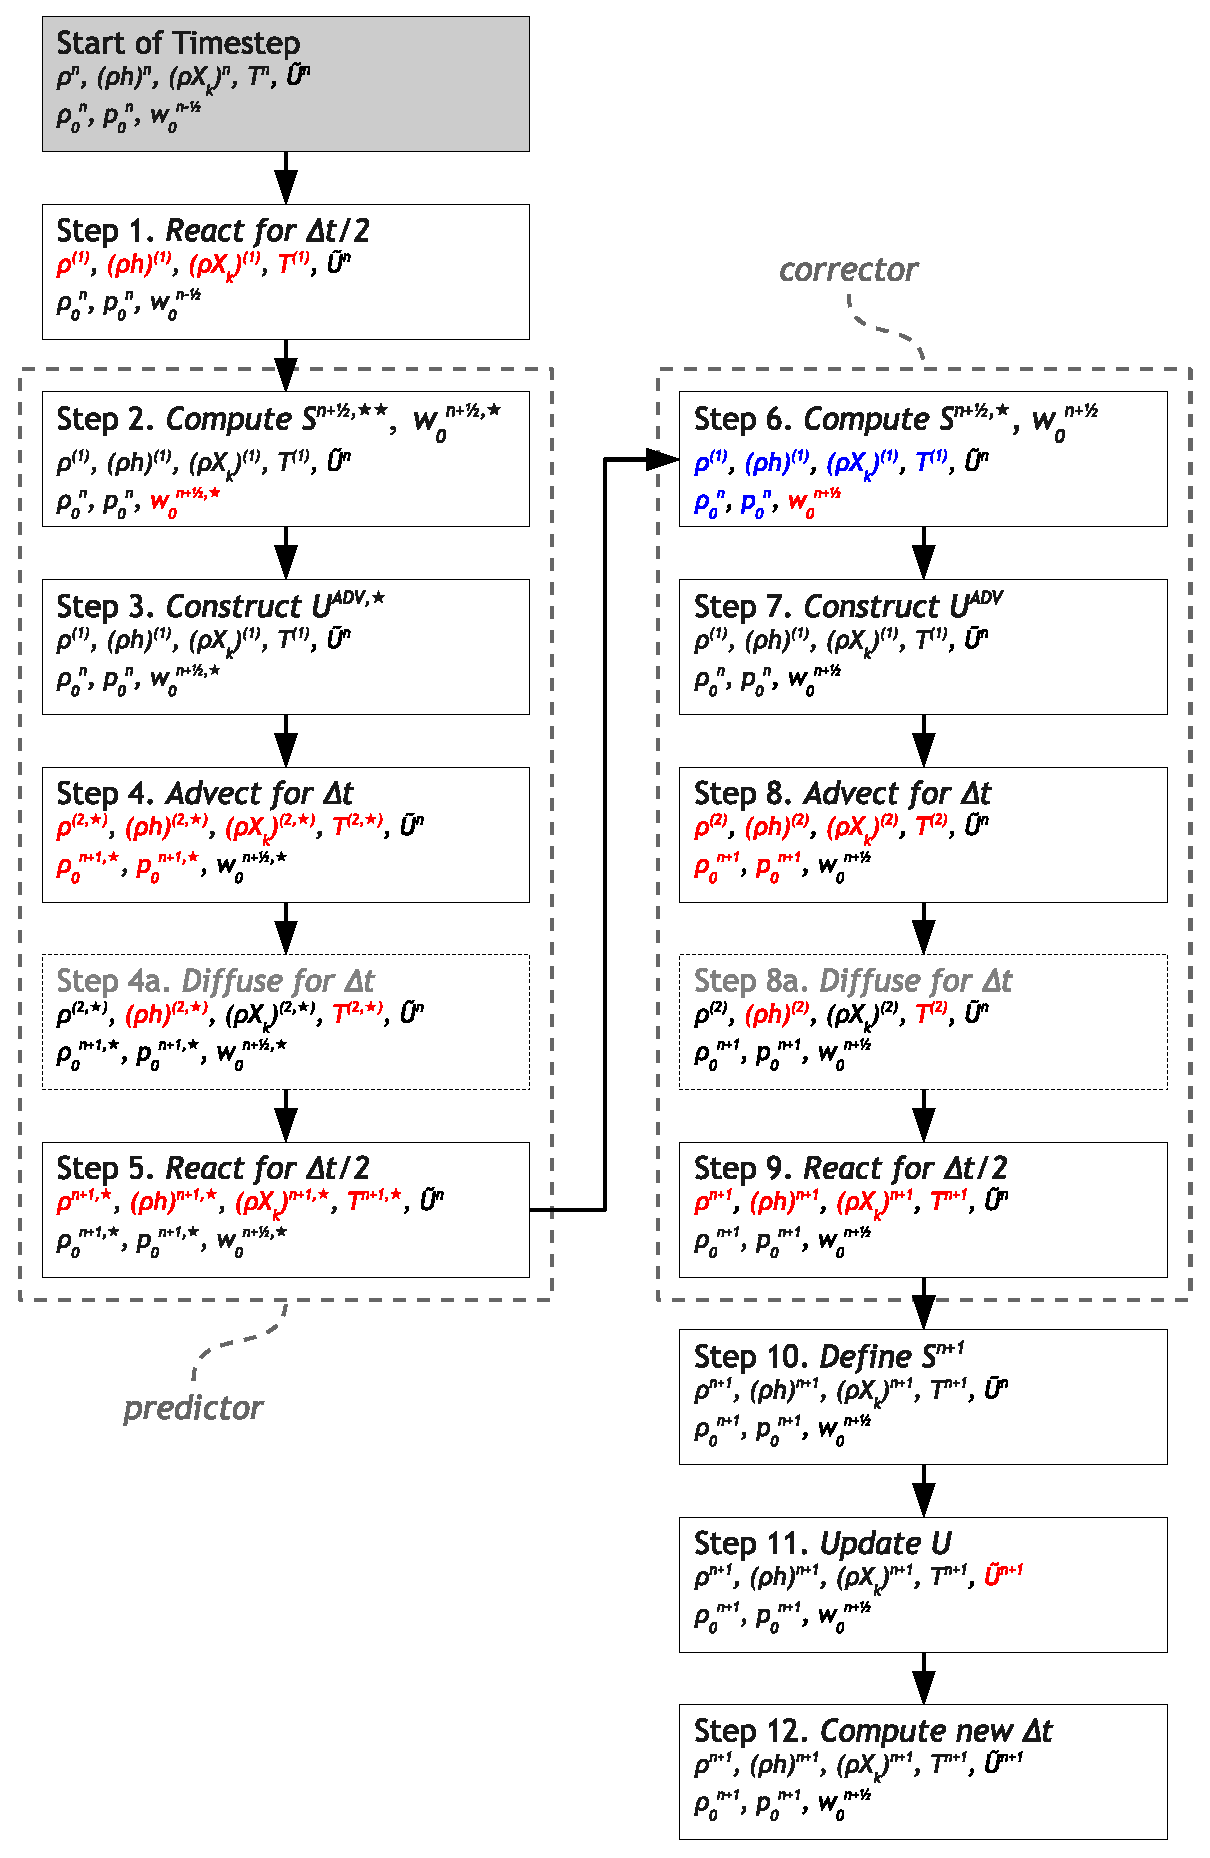
\includegraphics[scale=0.65]{\flowfigpath/flowchart}
\caption[Graphical flowchart of \maestro]
  {\label{Fig:flowchart} A flowchart of the algorithm.  The
  thermodynamic state variables, base state variables, and local velocity are
  indicated in each step.  Red text indicates that quantity was
  updated during that step.  The predictor-corrector steps are
  outlined by the dotted box.  The blue text indicates state
  variables that are the same in {\bf Step 6} as they are in
  {\bf Step 2}, i.e., they are unchanged by the predictor steps.
  The diffusion steps (4a and 8a) are optional, depending on
  {\tt use\_thermal\_diffusion}.}
\end{figure}
%%%%%%%%%%%%%%%%%%%%%%%%%%%%%%%%%
%%%%%%%%%%%%%%%%%%%%%%%%%%%%%%%%%
\begin{figure}[tb]                                               
\centering
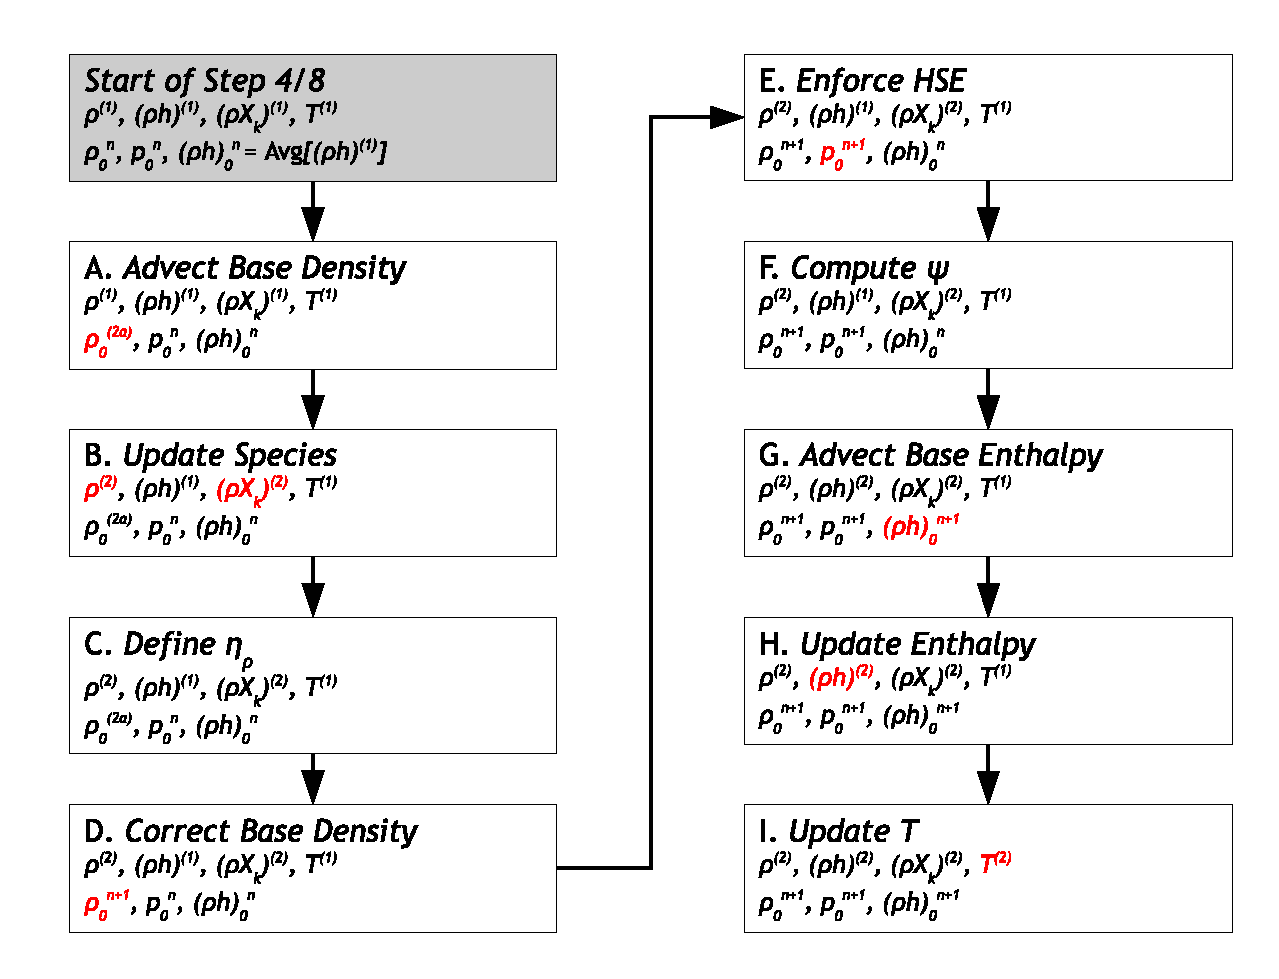
\includegraphics[scale=0.75]{\flowfigpath/flowchart_4_8}
\caption[Graphical flowchart of the density and enthalpy update steps]
{\label{Fig:flowchart48} A flowchart for {\bf Steps 4} and {\bf 8}.
  The thermodynamic state variables and base state variables are
  indicated in each step.  Red text indicates that quantity was
  updated during that step.  Note, for {\bf Step 4}, the updated
  quantities should also have a $\star$ superscript, e.g., {\bf Step
    8I} defines $T^{(2)}$ while {\bf Step 4I} defines $T^{(2),\star}$
  .}
\end{figure}


%-----------------------------------------------------------------------------
% Initialization
%-----------------------------------------------------------------------------

\section{Initialization}\label{Sec:Initialization}

\label{sec:flow:initialization}
 
We start each calculation with user-specified initial values for
$\rho$, $X_k$ and $T,$ as well as an initial background state.  In
order for the low Mach number assumption to hold, the initial data
must be thermodynamically consistent with the initial background
state.  In addition, the initial velocity field must satisfy an
initial approximation to the divergence constraint.  We use an iterative
procedure to compute both an initial right-hand-side for the
constraint equation and an initial velocity field that satisfies
the constraint.  The user specifies the number of iterations,
$N_{\rm iters}^{S},$ in this first step of the initialization procedure.

The initial perturbational pressure also needs to be determined for
use in {\bf Steps 3}, {\bf 7}, and {\bf 11}. 
This is done through a second iterative procedure which follows the
time advancement algorithm as described in {\bf Steps 1-11} in 
\S \ref{Sec:Time Advancement Algorithm}.  
The user specifies the number of iterations, 
$N_{\rm iters}^{\pi},$ in this second step of the initialization procedure.
The details for both iterations are given below.\\

%--------------------------------------------------------------------------
% STEP 0
%--------------------------------------------------------------------------
\noindent {\bf Step 0.} {\em Initialization}

First, we need to construct approximations to $S^0, w_0^{-\myhalf}, \Delta t^0$, 
and $\Ub^0$.  Start with initial data $X_k^{\initp}, \rho^{\initp},$ $T^{\initp},$ 
an initial base state, and an initial guess for the velocity, $\Ub^{\initp}$.
Set $w_0^0 = 0$ as an initial approximation.  Use the equation of state to 
determine $(\rho h)^{\initp}$.  Compute $\beta_0^0$ as a function of 
the initial data.  The next part of the initialization process 
proceeds as follows.

\begin{enumerate}
\renewcommand{\theenumi}{{\bf \alph{enumi}}}
\renewcommand{\labelenumii}{\roman{enumii}.}

\item {\em Initial Projection}: if {\tt do\_initial\_projection = T}, then we 
   first project the velocity field with $\rho = 1$ and $\beta_0^0$.
   The initial projection does not see reactions
   or external heating, and thus we set $\dot\omega = \Hnuc = \Hext = 0$ in $S$.
   The reason for ignoring reactions and heating is that we need some kind of 
   time scale over which to compute the effect of reactions, but we first 
   need an estimate of the velocity
   field in order to derive the time step that will be used as a time scale.
   The elliptic equation we solve is 
   \begin{equation}
   \nabla \cdot \beta_0^0 \nabla \phi = \beta_0^0(S - \Sbar)- \nabla \cdot (\beta_0^0 \Ub^{\initp})
   \end{equation}
   This $\phi$ is then used to correct the velocity field to obtain $\Ub^{0,0}$.
   If {\tt do\_initial\_projection = F}, set $\Ub^{0,0} = \Ub^{\initp}$.

\item {\em ``Divu'' iterations}: Next we do {\tt init\_divu\_iter} iterations 
  to project the velocity field using a constraint that sees reactions
  and external heating. 
  The initial timestep estimate is provided by {\tt firstdt} and
  $\Ub^{0,0}$, to allow us to compute the effect of reactions over $\Delta t/2$.

  {\bf Do} {$\nu = 1,...,N_{\rm iters}^{S}$.}
  \begin{enumerate}

  \item Estimate $\Delta t^\nu$ using $\Ub^{0,\nu-1}$ and $w_0^{\nu-1}.$

  \item {\bf React State}$[ \rho^{\initp},(\rho h)^{\initp}, X_k^{\initp}, T^{\initp}, 
(\rho^{\initp} \Hext), p_0^{\initp}] \rightarrow [\rho^{\outp}, (\rho h)^{\outp}, 
X_k^{\outp}, T^{\outp}, (\rho \omegadot_k)^{0,\nu} ].$

  \item Compute $S^{0,\nu}$ from equation (\ref{eq:defineS}) 
        using $(\rho \omegadot_k)^{0,\nu}$ and the initial data.

  \item Compute $\overline{S^{0,\nu}} = {\mathrm{\bf Avg}} (S^{0,\nu}).$

  \item Compute $w_0^{\nu}$ as in {\bf Step 2B} using $\overline{S^{0,\nu}}$ and $\psi=0$.
        
  \item Project $\Ub^{0,\nu-1}$ using $\beta_0^0$ and 
        $(S^{0,\nu} - \overline{S^{0,\nu}})$ as the source term.  
        This yields $\Ub^{0,\nu}.$  In this projection, again the density is 
        set to 1, and the elliptic equation we solve is:
   
   \begin{equation}
   \nabla \cdot \beta_0^0 \nabla \phi = \beta_0 (S - \Sbar)- \nabla \cdot (\beta_0^0 \Ub^{0,\nu-1})
   \end{equation}


  \end{enumerate}

  {\bf End do.}

  Define $S^0 = S^{0,N_{\rm iters}^S}$, $w_0^{-\myhalf} = w_0^{N_{\rm iters}^S}$, 
$\dt^0 = \Delta t^{N_{\rm iters}^S},$ and $\Ub^0 = \Ub^{0,N_{\rm iters}^S}.$

\end{enumerate}

Next, we need to construct approximations to $\etarho^{-\myhalf}, \psi^{-\myhalf}, S^1$,
and $\pi^{-\myhalf}$.  As initial approximations, set 
$\etarho^{-\myhalf}=0, \psi^{-\myhalf}=0, S^{1,0}=S^0$, and $\pi^{-\myhalf}=0.$
\begin{enumerate}
\renewcommand{\theenumi}{{\bf \alph{enumi}}}
\renewcommand{\labelenumii}{\roman{enumii}.}
\addtocounter{enumi}{2}
\item {\it Pressure iterations}: Here we do {\tt init\_iter} iterations to get an
  approximation for the lagged pressure:

  {\bf Do} {$\nu = 1,...,N_{\rm iters}^{\pi}$.}
  \begin{enumerate}
  \item Perform {\bf Steps 1-11} as described above, using 
    $S^{\myhalf,\star\star} = (S^0 + S^{1,\nu-1})/2$ in {\bf Step 2} as described.
    The only other difference in the time advancement is that in {\bf Step 11}
    we define ${\bf V} = (\Ubt^{1,\star} - \Ubt^0)$ and solve
    \begin{equation}  L_\beta^\rho \phi = D \left ( \beta_0^{\myhalf} {\bf V} \right) - \beta_0^{\myhalf} \left[ \left(S^{1}-\overline{S^{1}}\right) - \left(S^{0}-\overline{S^{0}}\right) \right] \enskip . 
    \end{equation}
    (The motivation for this form of the projection in the initial pressure iterations
    is discussed in \cite{almgren:bell:crutchfield}.)
      We discard the new velocity resulting from this, but keep the new  
      value for $\pi^{\myhalf} = \pi^{-\myhalf} + (1 / \dt) \; \phi.$  
      These steps also yield new scalar data at time $\dt,$ which
      we discard, and new values for $\etarho^{\myhalf}$ ({\bf Step 8C}), 
      $\psi^{\myhalf}$ ({\bf Step 8F}), 
      $S^{1,\nu}$ ({\bf Step 10A}), and $\pi^{\myhalf}$ ({\bf Step 11}), which we keep.
    \item Set $\pi^{-\myhalf} = \pi^{\myhalf}$, $\etarho^{-\myhalf} = \etarho^{\myhalf}$,
      and $\psi^{-\myhalf} = \psi^{\myhalf}$. 
    \end{enumerate}
    
    {\bf End do.}
    
    Finally, we define $S^1 = S^{1,N_{\rm iters}^\pi}.$
    
  \end{enumerate}

The tolerances for these elliptic solves are described in \S~\ref{sec:mgtol}.


%-----------------------------------------------------------------------------
% changes
%-----------------------------------------------------------------------------

\section{Changes from Earlier Implementations}
\subsection{Changes Between Paper 3 and Paper 4}
\begin{enumerate}
\item We defined the mapping of data between a 1D radial array and the 3D Cartesian
grid for spherical problems (which we improve upon in the multilevel paper).
\item We update $T$ after the call to {\bf React State}.
\item We have created a {\tt burning\_cutoff\_density}, where the burning does
not happen below this density.  It is presently set to {\tt base\_cutoff\_density}.
\item Use corner coupling in advection.
\item We have an option, controlled by {\tt use\_tfromp}, to update temperature 
using $T=T(\rho,X_k,p_0)$ rather than $T=T(\rho,h,X_k)$.  The former completely 
decouples enthalpy from our system.  For spherical problems, we use 
{\tt use\_tfromp = TRUE}, for planar problems, we use {\tt use\_tfromp = FALSE}.
\item For spherical problems, we have changed the discretization of 
$\Ubt\cdot\nabla p_0$ in the enthalpy update to 
$\nabla\cdot(\Ubt p_0) - p_0\nabla\cdot\Ubt$.
\item In paper III we discretized the enthalpy evolution equation in
terms of $T$.  Since then we have discovered that 
discretizing the enthalpy evolution in perturbational form, $(\rho h)'$,
leads to better numerical properties.  We use {\tt enthalpy\_pred\_type = 1}.
This is more like paper II.
\item We have turned off the evolution of $h$ above the atmosphere and instead
compute $h$ with the EOS using {\tt do\_eos\_h\_above\_cutoff = TRUE}.
\end{enumerate}


\subsection{Changes Between Paper 4 and the Multilevel Paper}
See the multilevel paper for the latest.


\subsection{Changes Between the Multilevel Paper and Paper 5}
\begin{enumerate}
\item Added rotation.
\end{enumerate}


\subsection{Changes Between Paper 5 and the XRB Paper}
\begin{enumerate}
\item We have added thermal diffusion, controlled by {\tt use\_thermal\_diffusion},
{\tt temp\_diffusion\_formulation}, and {\tt thermal\_diffusion\_type}.
\item We added the volume discrepancy term to the velocity constraint equation,
controlled by the input parameter, {\tt dpdt\_factor}.
\item For certain problems, we need to set {\tt do\_eos\_h\_above\_cutoff = FALSE}
to prevent large, unphysical velocities from appearing near the edge of the star.
\end{enumerate}

%-----------------------------------------------------------------------------
% Future Considerations
%-----------------------------------------------------------------------------

\section{Future Considerations}

\begin{itemize}
\item Should we use a predictor-corrector for updating the full-state density?
Specifically, after calling {\bf Correct Base}, should we do a full-state density 
advance and {\bf Correct Base} using the more accurate estimate of $\rho_0^{n+1}$?
\item We are still exploring the effects of {\tt use\_tfromp = FALSE} for spherical
problems.  We would eventually like to run in this mode, but $T=T(\rho,X_k,p_0)$ 
and $T=T(\rho,h,X_k)$ drift away from each other more than we would like.  Our
attempts at incorporating a {\tt dpdt\_factor} for spherical problems have not 
been successful.
\end{itemize}

